\documentclass{article}
\usepackage{graphicx}
\usepackage{setspace}
\usepackage{amsmath}
\usepackage{kbordermatrix}
\usepackage{graphicx}
\graphicspath{{latex_pictures/}}
\doublespacing

\begin{document}

\title{}
 
\author{Jesse Zhang}
 

 
\maketitle % this produces the title block
 
\begin{abstract}
If you use this template and follow the instructions therein,
your will be able to write a paper using LaTeX.
\end{abstract}

 
\section{Purpose}

The purpose of the parser is to take a phylogenetic tree via variations of Newick notation, and create a distance matrix based on the taxa given via the Unrooted STAR method(U-STAR). The parser was written in R. 

\section{File parser}
Each file given to the program will have two to three sections. The end of each section is denoted by the use of //.

The first section denotes whether or not the user will be using the alternate naming scheme for their Newick notation. This is to be set to TRUE or FALSE, more on the alternate naming scheme can be found at (references). 

After the program has determined whether or not you are using the alternate naming scheme it will then process the Newick notation line by line, turning them into a distance matrix. These distance matrices will then be stored into a list called {\tt distanceMatrixList}. If the alternate naming scheme is set to true we will store the species name before the $\_$ and have it with the associated taxa, more on this is explained in the third section.  

The third section of the file parser is only relevant if alternate naming scheme is set to FALSE. if so then the program will take line by line the species and the associated taxa forming a list of lists with each nested list having two values, the key and the associated taxa this is stored in the {\tt keyList}. Upon completing this it will list the associated species with the taxa and prompt the user if the results are acceptable or not.

Upon confirmation of acceptable results the program will then take the {\tt distanceMatrixList} and make a list of lists with the nested list having each {\tt distanceMatrixList} entry and a list of lists where the first value denotes each key and the second value is a with a one by $Y$ vector filled with zeros with $Y$ being the col length of {\tt distanceMatrixList} this list of lists is called the {\tt matrixKeyList}. We will then look to populate these one by $Y$ vector, this will be done by passing through the {\tt keyList} for each taxa found inside the associated distance matrix we set its appropriate index in the vector to one. This is done for all distance matrices and is stored in the {\tt matrixReductionList}. 

After all distance matrices have had an associated list of species, and ones denoting which entries of the distance matrix has the associated taxa we will then look to calculate the phylogenetic matrix based on the species. We initialize the {\tt phyloMatrix} a $Z$ by $Z$ matrix with $Z$ being the total amount of species (the length of {\tt keyList}). Its column names and row names will then have its names set to the key names to make for easier indexing. 

We populate the {\tt phyloMatrix} by examining all combinations of two species in the {\tt keyList} for each combination we take both associated 1 by $Y$ vectors and multiply it to the associated distance matrix in order to obtain all entries of the associated species added together. If this is equal to, the program will notify the user that one of the matrices/Newick notation does not contain all species and will exit out of the program. If not, the program will then divide this by the total amount of entries, which is the product of the sums of both associated 1 by $Y$ vectors. This process is then repeated for each distance matrix in the {\tt matrixReductionList}. These values are then summed then divided by the length of the {\tt matrixReductionList}. The program will then proceed to enter the appropriate phylogenetic tree length in the appropriate index in the {\tt phyloMatrix}

\section{Concept}

Given the Newick notation $(((A,B),C),(D,E))$ we wish to obtain the distance matrix:
\begin{figure}[!ht]
 \[
 \kbordermatrix{
	& A & B & C & D & E \\
	A & 0 & 2 & 3 & 4 & 4 \\
	B & 2 & 0 & 3 & 4 & 4 \\
	C & 3 & 3 & 0 & 3 & 3 \\
	D & 4 & 4 & 3 & 0 & 2 \\
	E & 4 & 4 & 3 & 2 & 0
}
\]
\caption{Distance matrix given the following Newick notation}
\end{figure}

In order to achieve this we determine which taxon to resolve first and form named nodes to help condense the Newick notation until we have two or three remaining taxa/node names. Visualizing the following Newick notation via a distance tree gives the following, with each branch having a length of one. \newline
\begin{figure}[!ht]
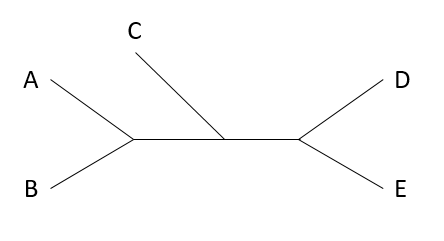
\includegraphics{firstTree.PNG}
\caption{Visualization of Newick notation as an unrooted tree}
\end{figure}
Based on the given Newick notation we wish to resolve the innermost taxon first, this is done by finding priority, which produces a table such as the one seen below.

\begin{figure}[!ht]
	\begin{center}
	\begin{tabular}{ |c|c| } 
		\hline
		Taxon/Node Name & Priority  \\
		\hline
		 A & 3 \\ 
		 \hline
		 B & 3 \\ 
		 \hline
		 C & 2 \\
		 \hline 
		 D & 2 \\
		 \hline 
		 E & 2 \\ 
		\hline
	\end{tabular}

	\end{center}
		\caption{Table with given priorities of the taxon/node names, higher priorities will be resolved first}
\end{figure}
As soon in \textit{fig. 3} we wish to resolve taxon A and B first, the resultant will be the creation of a named node with a distance vector from the taxa. This will reduce the tree removing A and B and instead replace both with a named node called tempVar0 as seen below. \newline

\begin{figure}[!ht]

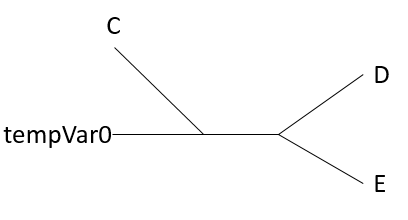
\includegraphics{secondTree.PNG} 
\caption{unrooted tree after two taxa have been condensed into a node name}
\end{figure}

Every node name has a distance vector associated with it, listing the distance away it is from relevant taxa, below is an example of that distance vector. 

\begin{figure}[!ht]
\[
\kbordermatrix{
	& \\
	A & 1 \\
	B & 1 \\
	C & 0 \\
	D & 0 \\
	E & 0
}
\]
\caption{tempvar0 associated distance vector}
\end{figure}

Any new node name will take upon the previous two taxa priority but have it reduced by one, this produces an updated priority table like so.

\begin{figure}[!ht]
\begin{center}
	\begin{tabular}{ |c|c| } 
		\hline
		Taxon/Node Name & Priority  \\
		\hline
		tempVar0 & 2 \\ 
		\hline
		C & 2 \\
		\hline 
		D & 2 \\
		\hline 
		E & 2 \\ 
		\hline
	\end{tabular}
\end{center}
\caption{updated priority table after two taxa have been condensed into a node name}
\end{figure}

The condensing of taxa/node names will continue to occur until there exist two or three remaining node names/taxa. The program then resolves the final nodes in a slightly different manner in order to produce the distance matrix seen in \textit{fig. 1}.

\section{Methodology}
 
\subsection{Setup Phase:}

This parser is limited to binary trees in Newick notation but allows for trees to be unrooted or rooted, with or without metric information.

When first given Newick notation, it will first remove all numeric data, leaving only the topological form of the tree. In order to remove numeric data, we pass through the input twice first removing branch lengths, related symbols, and extraneous whitespace. An example of this is given the Newick form $((AN3C:.1,B1ED:.2)123:.15,(CAS2:.1,DE4D:.05 )125:.2)$ it will be reduced to $((AN3C,B1ED),(CAS2,DE4D))$. 

Upon successfully simplifying the Newick notation, we extract all the taxa names as delimited by parentheses and commas they are then store them as a 1 by $X$ character array where $X$ is the number of taxa. The variable used to store these taxa is called {\tt myVars} and will be referenced multiple times through the program. 

After finding the taxa names we will initalize a list of lists called {\tt matrixList} with length $X$. Each {\tt matrixList} index has three parts, a taxon name({\tt var}), its priority({\tt value}) which is set to zero, and a 1 by $X$ distance vector. The 1 by $X$ vector will have its entries indexed by the taxon names with each initial entry being stored as a zero. {\tt value} slot will be used to decide what taxon to process first in the {\tt matrixList}.

After initialization of the {\tt matrixList} we will then determine priority for each taxon. We remove taxon names from the Newick notation temporarily replacing them white whitespace. For example $((A,B),C)$ becomes $((\_,\_),\_)$ this will allow us to ignore the taxa names in order to establish priority. We will read through this character by character. We initialize two variables that will be modified throughout, priority which is set to zero and count, which is set to one. If the char is a left parenthesis we increment the priority by one, if the char is a right parenthesis we decrease the priority by one. Finally, if the char is a whitespace we will store priority in the appropriate count index in {\tt matrixList} and increment count by one. Note, as {\tt myVars/matrixList} was initialized from left to right, the first whitespace on the left corresponds to the first matrixList index, the second whitespace corresponds to the second {\tt matrixList} index, and a similar pattern for the remaining whitespaces. The result is a {\tt matrixList} populated with their associated priority. 

The final distance matrix is initialized at this point as a $X$ by $X$ matrix. We will then set the column names and row names to the associated taxa names store in {\tt myVars}. 

\subsection{Algorithm}

Setting priority is important as we wish to compute the innermost taxa/node names first, for example in $((A,B),C)$. We would need to resolve A and B in a distance matrix before finally resolving it with taxa C. In order to do this the program will pass through {\tt matrixList} and identify taxon/node name with the highest priority, these will be stored by index in {\tt indexList} which is preallocated with the length of {\tt matrixList}. We will then proceed to process the leftmost values of {\tt indexList} two at a time. These values in {\tt indexList} represent the values in {\tt matrixList} that will be condensed. There exists three unique cases for condensing indexes in {\tt matrixList}, two taxa, one taxa and one node name, and two node names, in each case the two indexes must be handled differently.

\subsubsection{Case 1: two taxa}
In the case of two taxa the {\tt finalMatrix} will enter the taxa as having a distance of two apart. These taxa will then be deleted from {\tt matrixList} and be replaced by a node name. This node name will take on the previous taxas priority subtracted by one. The node name will also have its distance vector modified to have a one in the place of the two taxa that were removed from the {\tt matrixList}

\subsubsection{Case 2: one taxon and one node name}
In the case of one taxon one node name, the program will pass through the node names distance vector and for each index greater than zero it will enter that value plus two into the {\tt finalMatrix}. The index it fills in {\tt finalMatrix} is the one taxon and the associated index in the distance vector of the node name. Afterwards a new node name will be created with the former one taxon and one node name being deleted. The new node name will copy the old node names distance vector and increment each non-zero value by one, it will then set the appropriate index of the one taxon to one. As is similar in case 1 the new node name will have the previous one taxon one node name priority, but subtracted by one. 

\subsubsection{Case 3: two node name}
In the case of two node names the program passes through the first node name and for each non-zero value it will pass through the second node name for non-zero values. For each non-zero value in the second node name we will fill the {\tt finalMatrix} entry with the two non-zero values added together plus two. These two node names will then be deleted and replaced with a new node name taking on the previous priority subtracted by one. The distance vector of the new node name will have the two previous node name distance vectors added together. It will then increment any non-zero value in the distance vector by one. 

The program will continue passing through the {\tt matrixList} until its length is either three, with all three indexes having the same priority or if the length of the {\tt matrixList} is two. If there are only two remaining indexes a similar process is done as the above cases for populating values in the {\tt finalMatrix}, however rather then having the value plus two it is simply the value plus one. This is because there is no longer an additional branch to factor in due to it being the final two taxa/node names. 
However, in the case of the {\tt matrixList} having a length of three with each index having the same priority we have four unique cases, three taxa, two taxa and one node name, one taxa and two node names, and three node names. 

\subsubsection{Case 1: three taxa}

In this case of three taxa each taxon will have a distance of two apart from each other, and so the {\tt finalMatrix} will have six entries involving the associated pairing of taxa filled with the value two.

\subsubsection{Case 2: two taxa and one node name}

In the case of two taxa and one node name, we will identify the one node name and for each value in distance vector that is grater than zero we will take that value and add two to it and enter it into the {\tt finalMatrix} in the associated entries with that index and the two taxa. The remaining two entries between the two taxa will have a value of two.

\subsubsection{Case 3: one taxa and two node name}

In the case of one taxa and two node names we will create a temp distance vector of the two node names distance vector added together. If any value in the temp distance vector has a value greater than zero it will have its value entered in plus two into the {\tt finalMatrix} with the one taxa. With the remaining two node names will be resolved the exact same as case 3: two node name.

\subsubsection{Case 4: three node name}

For each non-zero value in the distance vector of the first node name we look for non-zero values in the second and third node node name. It will then combine these values plus two and enter it into the appropriate indexes of the {\tt finalMatrix}. A similar process is repeated between the second and third node names. 

After the last two/three indexes of the {\tt matrixList} has been resolved the program now has a completed {\tt finalMatrix} and will return {\tt finalMatrix}.

\end{document}


